We target a specific but very common use case. A researcher has written a paper with empirical content, and is required by the journal's data and code availability policy to prepare a ``replication package.'' The journal's policy requires that the code and data be accessible to others, but does not require deposit of the materials as a ``supplementary file,'' i.e., as a ZIP file on their website. However, in all cases, the journal wishes to ascertain three key attributes of the replication package or packages:
\begin{itemize}
    \item the existence of the package
    \item the access rules to the package (license, terms of use)
    \item the persistence of the package
\end{itemize}
In an ideal \ac{FAIR} and open-data compatible scenario, the existence of the package can be ascertained in a reputable repository, it is made available under an open license (e.g., CC-BY), and it is available ``forever''. These attributes, however, need to be discovered, and this needs to happen in a scalable, thus automated fashion, as it should be feasible to do so for all articles, submitted to any journal. 

\subsection{Use Case 1: public-use data}
In the first case, the researcher has  used public-use data, and identifies a \ac{DOI} to the journal (\url{http://doi.org/10.3886/E100590V1}). From this \ac{DOI}, the journal will attempt to identify the three attributes outlined above, using automated mechanisms. We thus start with the \ac{DOI}, which resolves to the following citation:

\lstset{numbers=left,numberstyle=\tiny,stepnumber=1,basicstyle=\linespread{0.8}\footnotesize}
\begin{quote}
	\it
McKinney, Kevin L., Green, Andrew S., Vilhuber, Lars, and Abowd, John M. Replication data: Total Error and Variability Measures for QWI and LODES. Ann Arbor, MI: Inter-university Consortium for Political and Social Research [distributor], 2017-12-15. https://doi.org/10.3886/E100590V1
\end{quote}

%We note that this dataset, as all current openICPSR datasets, is licensed under a \href{http://creativecommons.org/licenses/by/4.0/}{Creative Commons Attribution 4.0 International License}. 

\paragraph{DataCite}

We first query the DataCite API (Figure~\ref{fig:case1:datacite}).
\begin{figure}
\singlespacing
\lstinputlisting[language=xml,linerange=1-1]{supplementary_materials/datacite-api-100590.xml}
\lstinputlisting[language=xml,linerange=9-9,firstnumber=9]{supplementary_materials/datacite-api-100590.xml}
\lstinputlisting[language=xml,linerange=10-10,firstnumber=10,basicstyle=\bfseries\footnotesize]{supplementary_materials/datacite-api-100590.xml}
\lstinputlisting[language=xml,linerange=11-11,firstnumber=11]{supplementary_materials/datacite-api-100590.xml}
\lstinputlisting[language=xml,linerange=22-22,firstnumber=22]{supplementary_materials/datacite-api-100590.xml}
\lstinputlisting[language=xml,linerange=23-24,firstnumber=23,basicstyle=\bfseries\footnotesize]{supplementary_materials/datacite-api-100590.xml}
\caption{Select lines from DataCite query for DOI 10.3886/E100590V1}
\label{fig:case1:datacite}
\centering \footnotesize The full query response can be found in the appendix.
\end{figure}
%
The query reveals the identity of the \texttt{datacentre} and the \texttt{publisher}. However, there is no information on the license under which the object is made available, no copyright, license, or terms of use information, nor any information on persistence of the data. The \texttt{license} attribute is optional as per DataCite Schema \parencite{DataCiteMetadataWorkingGroupDataCiteMetadataSchema2017}, and is empty here.
 
\paragraph{re3data}
We turn to re3data for further information, and find two possible problems. A lookup for the contents of the \texttt{datacentre} field yields 0 results. A search for the contents of the \texttt{publisher} field yields a wrong result (\lstinline|<odesi>|). We applied human judgment to find a re3data record for ICPSR: \url{https://www.re3data.org/repository/r3d100010255} \parencite{Re3data-icpsr}. We note, however, that the rules and policies for openICPSR may differ from \urlcite{https://www.openicpsr.org/openicpsr/faqs}{ICPSR}.
The re3data record lists three types of data access. Furthermore, three data licenses are listed: two \texttt{other} and one \texttt{copyright}.
\begin{figure}[H]
	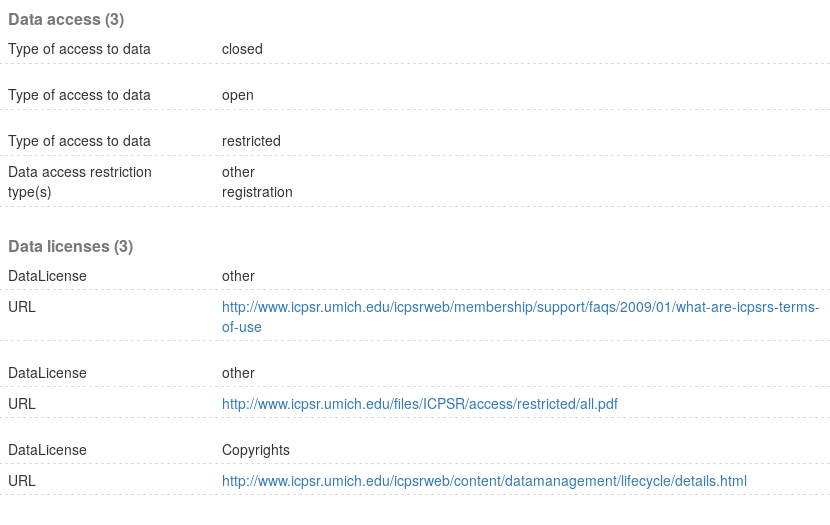
\includegraphics[width=1\textwidth]{supplementary_materials/re3data-org-icpsr-access-licenses-20181008.png}
	%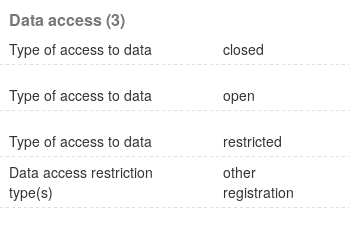
\includegraphics[width=0.4\textwidth]{re3data-org-icpsr-access-20181008.png}
\end{figure}
Thus, while re3data does contain entries of \textit{possible} licenses, we have no information on which one applies to the replication package above. Furthermore (not displayed here), there is no machine-readable information on persistence. While knowledgable data archivists and librarians, as well as many social scientists, ``know'' that ICPSR is a reputable archive with a long history and presumably a long future, this is not encoded anywhere where non-domain experts could ascertain it.

\paragraph{CoreTrustSeal}
We do not investigate whether this information is available on through CoreTrustSeal, for three reasons. First, searching again, as we did, through the website, neither of the search terms that the DataCite record provides yield findable results. Second, when we manually identify ICPSR on the website's map of institutions, we observe that ICPSR had a ``Data Seal of Approval'' (the predecessor to CoreTrustSeal), but that it expired in 2017, which may explain the lack of search results. Finally, the CoreTrustSeal certification is encapsulated in PDFs, and does not provide an API to search for attributes of a certified repository. While it may be feasible for a human to track down the relevant information, it is not scalable.

\paragraph{Data publisher website}
\newcommand{\icpsrdate}{8 October 2018}
\begin{figure}
\lstinputlisting[language=xml]{supplementary_materials/extract-webpage-20181008.xml}
    \caption{Use Case 1, Encoding of license in HTML of landing page}
    \label{fig:case1:rela}
\end{figure}
\begin{figure}
    \centering
    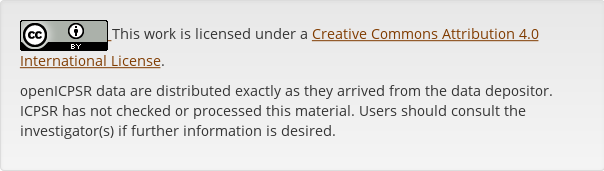
\includegraphics[width=0.5\linewidth]{images/openicpsr-license-image.png}
    \caption{Use Case 1, license as displayed on website on \icpsrdate }
    \label{fig:case1:license}
\end{figure}
Finally, we attempt to obtain metadata   directly from the landing page indicated by the \ac{DOI}.%
\footnote{The query was run on \icpsrdate .}
The page offers five types of metadata: the in-page metadata in XML format, in-page metadata encoded as JSON-LD, a link to a OAI-PMH record, a link to a DDI 2.5 record, and a link to a DDI 3.1 record.
The webpage provides two instances of license information. The first instance is within the \texttt{rel} identifier within the \lstinline|a| link field (Figure~\ref{fig:case1:rela}) with an associated displayed  license badge (Figure~\ref{fig:case1:license}).
The second instance is encoded in the JSON-LD payload,
\begin{lstlisting}
"license":"https://creativecommons.org/licenses/by/4.0/deed.en_US"
\end{lstlisting}
Both provide the same information about the license.


\paragraph{Conclusion on Use Case 1}
Additional information about the accessibility is not provided, even though ICPSR does provide data with more restrictive access rules, for instance, through secure cloud instances. Furthermore, no information is provided  about persistence. The openICPSR FAQ contain such information, but do so somewhat obliquely, and do not point to a policy. Browsing the website, one might encounter the ``\href{https://www.icpsr.umich.edu/icpsrweb/content/datamanagement/preservation/policies/index.html}{Digital Preservation Policies and Planning at ICPSR}'' \parencite{icpsr-preservation}, which  lays out the policies. 

We note that DataCite, while providing a means to communicate the license, did not do so at this time. DataCite does not provide a means to convey access rules or persistence, nor does it provide a means to point to specific policies on re3data. Re3data, in turn, lists three possible licenses, none of which apply in the present case, possibly because it lists information on the main ICPSR repository, and not on the associated but distinct openICPSR instance.

In this relatively straightforward case, we would need to query the user  about which license, and which access policy, applies to the particular dataset at hand. Alternatively, one could refer to a  list of ``vetted'' repositories, which may have checked most of the criteria that were not easily discernible. 

\subsection{Use Case 2: Restricted-access Data}

TODO: Use example from Census Bureau, backup policy of user files is 10 years (only known verbally), whereas the retention policy for input files is defined by official record schedules.

\subsection{Common Denominator}
We note that we chose plausible cases where the metadata crawl did not yield satisfactory information. For both data repositories, examples could have been chosen where the metadata might have yielded more satisfactory results. However, the methods of collecting the information must accommodate all scenarios, including the ones where the automated mechanisms fail.

We accomplish this by designing a derivative metadata package that can be populated at the point of first use: the journal submission system, or if the researcher uses a reproducible workflow, at data acquisition by the researcher. An associated light query system can first exhaust all metadata crawls, and pre-fill any fields. However, when ambiguous responses are obtained (as in Use Case 1), or no information is available (as in both use cases), the researcher can provide guided or verbatim answers. At both points in time, the researcher has the best incentives to provide the information accurately -- the acceptance of the submission may depend on the accuracy of the information -- and the most timely recollection of where to obtain the information.


\subsection{Why we cannot use the current infrastructure}
Examples here: see the supplementary materials: license information incomplete (DataCite), retention policy incomplete (re3data), links incomplete (Scholix). These may all become complete, but currently are not. Journals are implementing their replication policies now, and need the information now.